\documentclass{article}

\usepackage{geometry}
\usepackage{makecell}
\usepackage{array}
\usepackage{multicol}
\usepackage{setspace}
\usepackage{changepage}
\usepackage{booktabs}
\usepackage{graphicx}
\usepackage{cprotect}
\usepackage{float}
\newcolumntype{?}{!{\vrule width 1pt}}
\renewcommand\theadalign{tl}
\newcommand{\paragraphlb}[1]{\paragraph{#1}\mbox{}\\}
\setstretch{1.10}
\setlength{\parindent}{0pt}

\geometry{top=12mm, left=1cm, right=2cm}
\title{\vspace{-1cm}Betriebssysteme 1}
\author{Andreas Hofer}

\begin{document}
	\maketitle
	\section{Einheit 1 - 14.10.2024}
	Betriebssysteme sind gründsätzlich nur vonnöten, wenn mehrere Programme gleichzeitig auf die Hardware zugreifen sollen und das Betriebssystem dient als Mediator zwischen der Software. Zum Beispiel benötigte Leibniz' Rechenmaschine kein Betriebssystem, da es nur die vier Grundrechnungsarten beherrschte. Mit dem IBM 7090 von 1955 wurde die erste grundlegende Mediation der Programme eingeführt, was jedoch auch nicht als Betriebssystem gilt, als Batch Processing verwendet wurde um mehrere Programme konsekutiv (jedoch noch nicht gleichzeitig) auszuführen. Die Aufträge warten so in einer Schlange, und werden einer nach dem anderen abgearbeitet. Dabei unterstützten ein Vor- und Nachrechner das System um das Program zu laden und danach auszugeben. \\
	Ab den 1960ern wurden erste Systeme gebaut, welche Multitasking unterstützen. Dabei ist es strikt gesehen kein wahres multitasking, da oft nur eine CPU zur Verfügung stand und so jede Anfrage in kleinen Teilen abarbeitet. 
	\subsection{Abstraktionsebenen eines Rechensystems}
	Ein System hat mehrere Abstraktionsebenen um Anwendungen wiederzugeben:
	\begin{itemize}
		\item{Transistorebene}
		\begin{itemize}
			\item{Die unterste Ebene, in welcher Logik physisch mittels Schaltern wiedergegeben wird.}
		\end{itemize}
		\item{Gatterebene}
		\begin{itemize}
			\item{Eine abstrahierte Version der Schalter}
		\end{itemize}
		\item{Maschinenprogramme}
		\begin{itemize}
			\item{Logik, wiedergegeben durch Einsen und Nullen}
		\end{itemize}
		\item{Assemblerprogramme}
		\begin{itemize}
			\item{Mnemonische Repräsentationen des Maschinencodes}
		\end{itemize}
		\item{Anwendungsprogramm}
		\begin{itemize}
			\item{Programmcode wie C und Java}
		\end{itemize}
	\end{itemize}
	Ein Betriebssystem ist zwar Software, jedoch keine Anwendungssoftware. Anwendungssprogramme sind die eigentlichen Programme, welche als Benutzer ausgeführt werden wollen und Betriebssoftware ermöglicht diese Ausführung. Betriebssoftware ist so das Betriebssystem selbst, aber auch Treiber und andere Software, welche die Kommunikation zwischen der Hardware und der Software ermöglicht. \\
	Ein Betriebssystem bildet so einen zusätzliche Softwareschicht zwischen der Hardware und der Anwendungssoftware, sodass das Anwendungsprogramm nicht die Details der Hardware kennen muss um, zum Beispiel etwas zu speichern. \\
	\subsection{Abstraktion}
	Eine der grundlegenden Aufgaben eines Betriebssystems ist die Abstraktion. Dieses bietet eine abstrakte Sicht auf die Hardware und Software muss nicht wissen welche CPU vorhanden ist oder welche Festplatte eingebaut ist. Die Anwendung sendet eine Anfrage an das Betriebssystem, dass etwas abgespeichert werden muss, und das Betriebssystem kümmert sich um den Rest \\
	\subsection{Ressourcenverwaltung}
	Ressourcen in einem System wollen oft gleichzeitig von mehreren Programmen verwendet werden. Das Betriebssystem muss verwalten, dass Speicher nicht mehrfach verwendet oder die CPU nicht gleichzeitig mehrere Aufgaben abarbeiten soll. \\
	\subsubsection{Dienste}
	Ein Betriebssystem hat mehrere Dienste um einen reibungslosen Ablauf zu garantieren. \\
	\begin{itemize}
		\item{Prozessverwaltung}
		\begin{itemize}
			\item{Teilt Prozesse zeitlich ein, sodass diese von der CPU ausgeführt werden. Überwacht auch Speicherzugriffe und die Kommunikation zwischen Prozessen.}
		\end{itemize}
		\item{Speicherverwaltung}
		\begin{itemize}
			\item{Verwaltet den Hauptspeicher (RAM) und stellt sicher, dass ein Programm sich komplett im Speicher befindet, bevor es aufgeführt wird. Ist auch für die Virtualisierung des Speichers verantwortlich.}
		\end{itemize}
		\item{Dateiverwaltung}
		\begin{itemize}
			\item{Abstrahiert das Dateisystem zu Verzeichnissen und bildet dieses als Hierarchie ab. Es ist auch für Zugriffskontrolle verantwortlich und stellt sicher, dass nur Nutzer mit den nötigen Rechten Sachen ausführen.}
		\end{itemize}
		\item{Geräteverwaltung}
		\begin{itemize}
			\item{Initiiert, überwacht und verwaltet Peripheriegeräte. Diese sind nicht nur Maus, Tastatur und Bildschirm sondern auch Festplatten.}
		\end{itemize}
		\item{Benutzerschnittstelle}
		\begin{itemize}
			\item{Zusätzlich zu diesen grundlegenden Services gibt es auch noch die Schnittstelle damit ein Benutzer mit dem PC interagieren kann. Das kann entweder in Form eines Terminals (Einer CLI) oder einer grafischen Benutzeroberfläche (GUI) geschehen. Der große Vorteil der CLi ist hierbei die Möglichkeiten Abläufe zu automatisieren.}
		\end{itemize}
	\end{itemize}
	\subsection{Kernel-/Benutzermodus}
	Da das Betriebssystem trotzdem Software ist, benötigt es spezifische Priviliegien um seiner Aufgab nachkommen zu können. So gibt es zwei Zugriffsmodi: Kernelmodus und Benutzermodus. \\
	Der Kernelmodus hat grundsätzlich keine Zugriffsbeschränkungen und darf auch auf Speicherbereiche zugreifen, welche nicht dem Programm gehören (Da diese Programm ja nur über das Betriebssystem den Speicher verändern kann). Der Kernelmodus muss sicher und geschützt vor anderen Anwendungen sein, damit dieser nicht missbraucht werden kann. \\
	Der Benutzermodus ist der unprivilegierte Modus und hat nur eingeschränkten Zugriff.
	\subsection{Kernelarchitekturen}
	\subsubsection{Minimaler Kernel / Microkernel}
	Ein Microkernel implementiert nur die wichtigsten Teile im Kernelmodus und lässt andere, weniger wichtige Komponenten wie Geräte- und Dateisystemtreiber im Benutzermodus. Dadurch ist es sicherer und Komponenten sind auch einfacher auszutauschen, jedoch ist es auch langsamer, da mehr calls zum Kernel notwendig sind. Symbian, das betriebssystem alter Nokiahandys, verwendete einen Microkernel.
	\subsubsection{Monolithischer Kernel}
	Das Gegenteil dazu ist der monolithische Kernel. Hierbei sind alle Systemkomponenten Teil des Kernelmodus. Dadurch ist es bedeutend schneller, da jede der Komponenten direkt auf die Hardware zugreifen kann. Jedoch ist die Entwicklung eines solchen Kernels bedeutend aufwendiger, da jeder der Komponenten volle Rechte hat und dadurch hohe Sicherheitsanforderungen hat. Das System ist auch im Falle eines Fehlers nicht mehr in der Lage sich zu erholen und muss neugestartet werden.
	\subsubsection{Hybrider Kernel}
	Ein Hybrider Kernel versucht die Vor- und Nachteile der beiden Architekturen zu vereinen. Es ist jedoch nicht fixiert, welche Teile dadurch im Kernelmodus laufen und welche nicht. In der Regel sind hybride Kernel jedoch stabiler und sicherer als ein monolithischer Kernel, und schneller und weniger Programmieraufwand als ein Microkernel. Heutzutage laufen die meisten PCs mit einem Hybriden Kernel, da sowohl Windows als auch die neusten Versionen von MacOS diesen verwenden.
	\subsection{Maschinenbefehle}
	Maschinenbefehle sind Bitfolgen, welche codierte Instruktionen an den Prozessor sind. Der Befehlssatz ist hierbei die Menge der ausführbaren Befehle auf einem spezifischen Prozessor (x86, ARM, MIPS). Dadurch ist die Funktionalität bei Maschinenbefehlen in großem Maße von der CPU abhängig. \\
	Diese Bitfolgen werden jedoch von einem Benutzer nie direkt gesehen. Programmiert wird größtenteils in höheren Programmiersprachen wie Java oder C, aber auch der hardwarenahen Assemblersprache. Während der Code von C zuerst von einem Interpreter in Maschinencode übersetzt werden muss und C auf jedem System in etwas gleich funktioniert, hängt Assembler von der CPU ab. Da Assembler so weniger Übersetzung benötigt und die Übersetzung nicht geschieht, kann man selbst entscheiden wie etwas implementiert wird und Funktionen meist effizienter auszuführen. So werden sehr hardwareintensive Programme in Assembler geschrieben. Dabei gibt man jedoch keine Bitfolgen an, sondern mnemonische Wortfolgen wie: \verb|ADD EAX, F16|. Dieser Befehl addiert zum Beispiel zwei Zahlen. So besteht jeder Befehl aus einem OP-Code und ein oder zwei Operanden.
	\subsubsection{Befehlsarten}
	Es gibt mehrere Arten von Befehlen: 
	\begin{itemize}
		\item{Transportbefehle}
		\begin{itemize}
			\item{Weisen das System zur Speicherung/Ladung eines Werts in einer spezifischen Zelle an.}
			\item{Z.B. \verb|LOAD STORE| }
		\end{itemize}
		\item{Arithmetische/Logische Befehle}
		\begin{itemize}
			\item{Befehle zur Ausführung von beispielsweise Addition oder Subtraktion}
			\item{Z.B. \verb|ADD SUB MUL DIV| }
		\end{itemize}
		\item{Sprungbefehle}
		\begin{itemize}
			\item{Befehle werden normalerweise sequenziell abgearbeitet, jedoch kann man die CPU anweisen zu einer anderen Zelle oder Flag zu springen.}
			\item{Z.B. \verb|JMP JNE| }
		\end{itemize}
	\end{itemize}
	\subsubsection{Von Neumann Zyklus}
	Der von Neumann Zyklus beschreibt die Abfolge der Ausführung eines Befehlscodes:
	\begin{enumerate}
		\item{Fetch}
		\begin{itemize}
			\item{Lädt den Befehl aus dem Speicher anhand des Zählers in das Register und erhöht den Zähler}
		\end{itemize}
		\item{Decode}
		\begin{itemize}
			\item{Verwendet die Befehlstabelle um herauszufinden was zu tun ist.}
		\end{itemize}
		\item{Execute}
		\begin{itemize}
			\item{Führt den angegeben Befehl aus.}
		\end{itemize}
	\end{enumerate}
	\subsection{CISC vs RISC}
	CPUs kann man in zwei Gruppen von Instruktionen klassifizieren: CISC und RISC
	\begin{itemize}
		\item{CISC}
		\begin{itemize}
			\item{Complex Instruction Set Computers (CISC) haben viele komplexe Instruktionen, welche oft mehrere Takte für die Ausführung eines Befehls benötigen. Zum Beispiel kann man in CISC zwei Zahlen direkt aus dem Arbeitsspeicher addieren. Sie haben auch Maschinencodes variabler Länger und besitzen meist weniger Registerplätze.}
		\end{itemize}
		\item{RISC}
		\begin{itemize}
			\item{Reduced Instruction Set Computer (RISC) haben im Gegensatz wenige simple Instruktionen. In der Regel sollten alle Befehle in einer RISC Architektur in nur einem Takt abgearbeitet werden können. Jeder Maschinencode hat auch die gleiche Länge und da jede Speicherung dezidiert erfolgen muss, hat es auch mehr Registerplätze.}
		\end{itemize}
	\end{itemize}
	\subsection{Prozessverwaltung}
	Prozesse sind Abstraktionen von ausgeführten Programmen. Während ein Programm eine Folge von Anweisungen und die dazugehörigen Daten sind, ist ein Prozess dieses Programm in Ausführung ist. Alle Zähler, Reigsterinhalte und Variablenbelegungen werden dabei auch im Prozess festgehalten. So ist ein Prozess die gesamte Ausführungsumgebung eines Programms. Ein Prozess kann auch mehrmals auf dem gleichen System unabhängig voneinander laufen. Da ein Prozess ein Programm in Ausführung ist braucht dieses auch gewisse Ressourcen. Prozessresourcen sind oft unter anderem die CPU, Speicher und Dateien. Das Betriebssystem abstrahiert dabei die Prozessausführung sodass viele Prozesse gleichzeitig ausgeführt werden können. \\
	\paragraphlb{Prozessmanager}
	Dabei reguliert der Prozessmanager die Interaktion zwischen Prozessen. Ein Prozessmanager hat grundlegende Aufgaben wie das Erstellen und Löschen von Benutzer- und Systemressourcen. Er ist auch dafür verantwortlich dafür Prozesse anzuhalten und fortzusetzen sowie Prozesse zu synchronisieren. Prozesse müssen synchron sein, um sicherzustellen, dass ein Prozess, welcher von einem anderen abhängt diesen auch erst danach ausführt. Ein Prozessmanager hat einen Scheduler, um Prozesse zu starten und zu beenden und einen Dispatcher um Prozesse zu wechseln (Context Switching).
	\paragraphlb{Singletasking/Multitasking}
	Da eine CPU grundsätzlich zu jedem Zeitpunkt nur einen Prozess bearbeiten kann, ist es nötig dessen Arbeit aufzuteilen. \\
	Bei dem Singletasking werden Prozesse hintereinander ausgeführt. \\
	Bei dem Multitasking werden mehrere CPU Kerne verwendet um mehrere Aufgaben gleichzeitig zu bearbeiten, jedoch kann man mittels Quasiparallelität auch bei nur einem CPU Kern gleichzeitig mehrere Prozesse ausführen. Dabei wechselt die CPU sehr schnell zwischen verschiedenen Prozessen und jeder der Prozesse bekommt nur einen Bruchteil der Rechenzeit, wodurch die Illusion entsteht, dass es gleichzeitig abläuft. \\
	\subsubsection{Prozessmodell}
	Ein Prozess hat grundsätzlich kein Wissen über den Status des Systems. Laut der Ansicht des Prozesses hat er jegliche CPU Zeit und den gesamten RAM Speicher zur Verfügung und das Betriebssystem gibt dabei nur die Resourcen frei, die der Prozess benötigt. Jeder Prozess hat auch seinen eigenen Prozesszähler um sich merken zu können, wo der Prozess das letzte Mal aufgehört hat. Wenn ein Prozess ausgeführt wird, wird dem Prozess ein Prozessraum zugewiesen, was Speicher ist, welcher für diesen Prozess reserviert ist.
	\paragraphlb{Adressraum}
	Ein Programm benötigt innerhalb des Speichers eine gewisse Menge an Speichern:
	\begin{itemize}
		\item{Den Wert des Befehlszählers}
		\item{Den Inhalt der zum Prozess gehörenden Prozess-Register}
	\end{itemize}
	Zusätzlich werden 4 Segmente im Speicher reserviert:
	\begin{enumerate}
		\item{Text - Speichert das Programmsegment (Der ausführbare Code)}
		\item{Datensegment - Speichert globale Variablen}
		\item{Stack - Speichert temporäre Daten}
		\item{Heap - Speichert dynamisch angeforderten Code}
	\end{enumerate}
	\paragraphlb{Prozesserzeugung}
	Ein Prozess kann auf mehrere Wege erzeugt werden:
	\begin{itemize}
		\item{Bei der Initialisierung des Systems}
		\begin{itemize}
			\item{Wenn im Vordergrund: Verlangen Benutzereingabe}
			\item{Wenn im Hintergrund(Daemons/Dienste): Erfordern keine Interaktion}
		\end{itemize}
		\item{Benutzeranfrage zur Erzeugung eines neuen Prozesses}
		\begin{itemize}
			\item{Beim Starten einer Benutzerandwendung (Zum Beispiel durch einen Doppelklick)}
		\end{itemize}
		\item{Systemaufrufe zur Erzeugung eines neuen Prozesses}
	\end{itemize}
	Wenn ein anderer Prozess einen Prozess erstellt, ist dieser Hierarchisch diesem untergeordnet. Dabei wird jedem Prozess eine Process-ID (PID) zugeordnet um diese zu identifizieren. Solche Hierarchien bestehen jedoch nur in Linux und MacOS (Unix Systemen) während in Windows alle Prozesse gleichwertig sind.
	\subsubsection{Unterbrechungen}
	\paragraphlb{System Calls}
	Ein Prozess, welcher im User Mode läuft hat keinen Zugriff auf Kernel-Level Funktionen. Wenn ein Prozess jedoch eine Funktion benötigt, für welche er keine Autorität besitzt, kann dieser mittels System Call eine Anfrage an das Betriebssystem ausgeben. \\
	Wenn so ein System Call ausgeht, unterbricht das Betriebssystem die Ausführung des Programms und übernimmt die Prozesszeit um die Anfrage abzuarbeiten. Dabei wird zu einer Kernel Service Routine gewechselt, welche den System Call bearbeiten kann. Nachdem die KSR abgeschlossen ist wird die Kontrolle wieder an das User Mode Programm zurückgegeben und es kann weiter ausgeführt werden. \\
	Für System Calls besteht der sogenannte POSIX Standard (Portable Operating System Interface) durch welchen die System Calls standardisiert werden können, sodass zum Beispiel 'open' stets eine Datei zum Lesen/Schreiben öffnet. Der POSIX Standard ist jedoch nicht allzu weit verbreitet. Während Mac OS POSIX konform ist, ist Linux nur teilweise konform und Windows definiert seinen eigenen Standard. Das bedeutet nicht, dass es in Linux oder Windows keinen 'open' command gibt, jedoch ist dieser eventuell unterschiedlich.
	\paragraphlb{Hardware Interrupt}
	Es gibt auch Hardwareunterbrechungen, welche Events sind die durch eine Hardwarekomponente ausgelöst werden. Zum Beispiel registriert das Betriebssystem bei jedem Tastendruck auf der Tastatur eine Unterbrechung um diesen Druck zu verarbeiten.
	\paragraphlb{Exception}
	Wenn ein Fehler auftritt, kann das Betriebssystem auch die Kontrolle übernehmen. Das passiert zum Beispiel, wenn man in einem Programm eine Speicherverletzung hat (Segmentation Fault).
	\subsubsection{Prozesszustände}
	\begin{figure}[H]
	\centering
	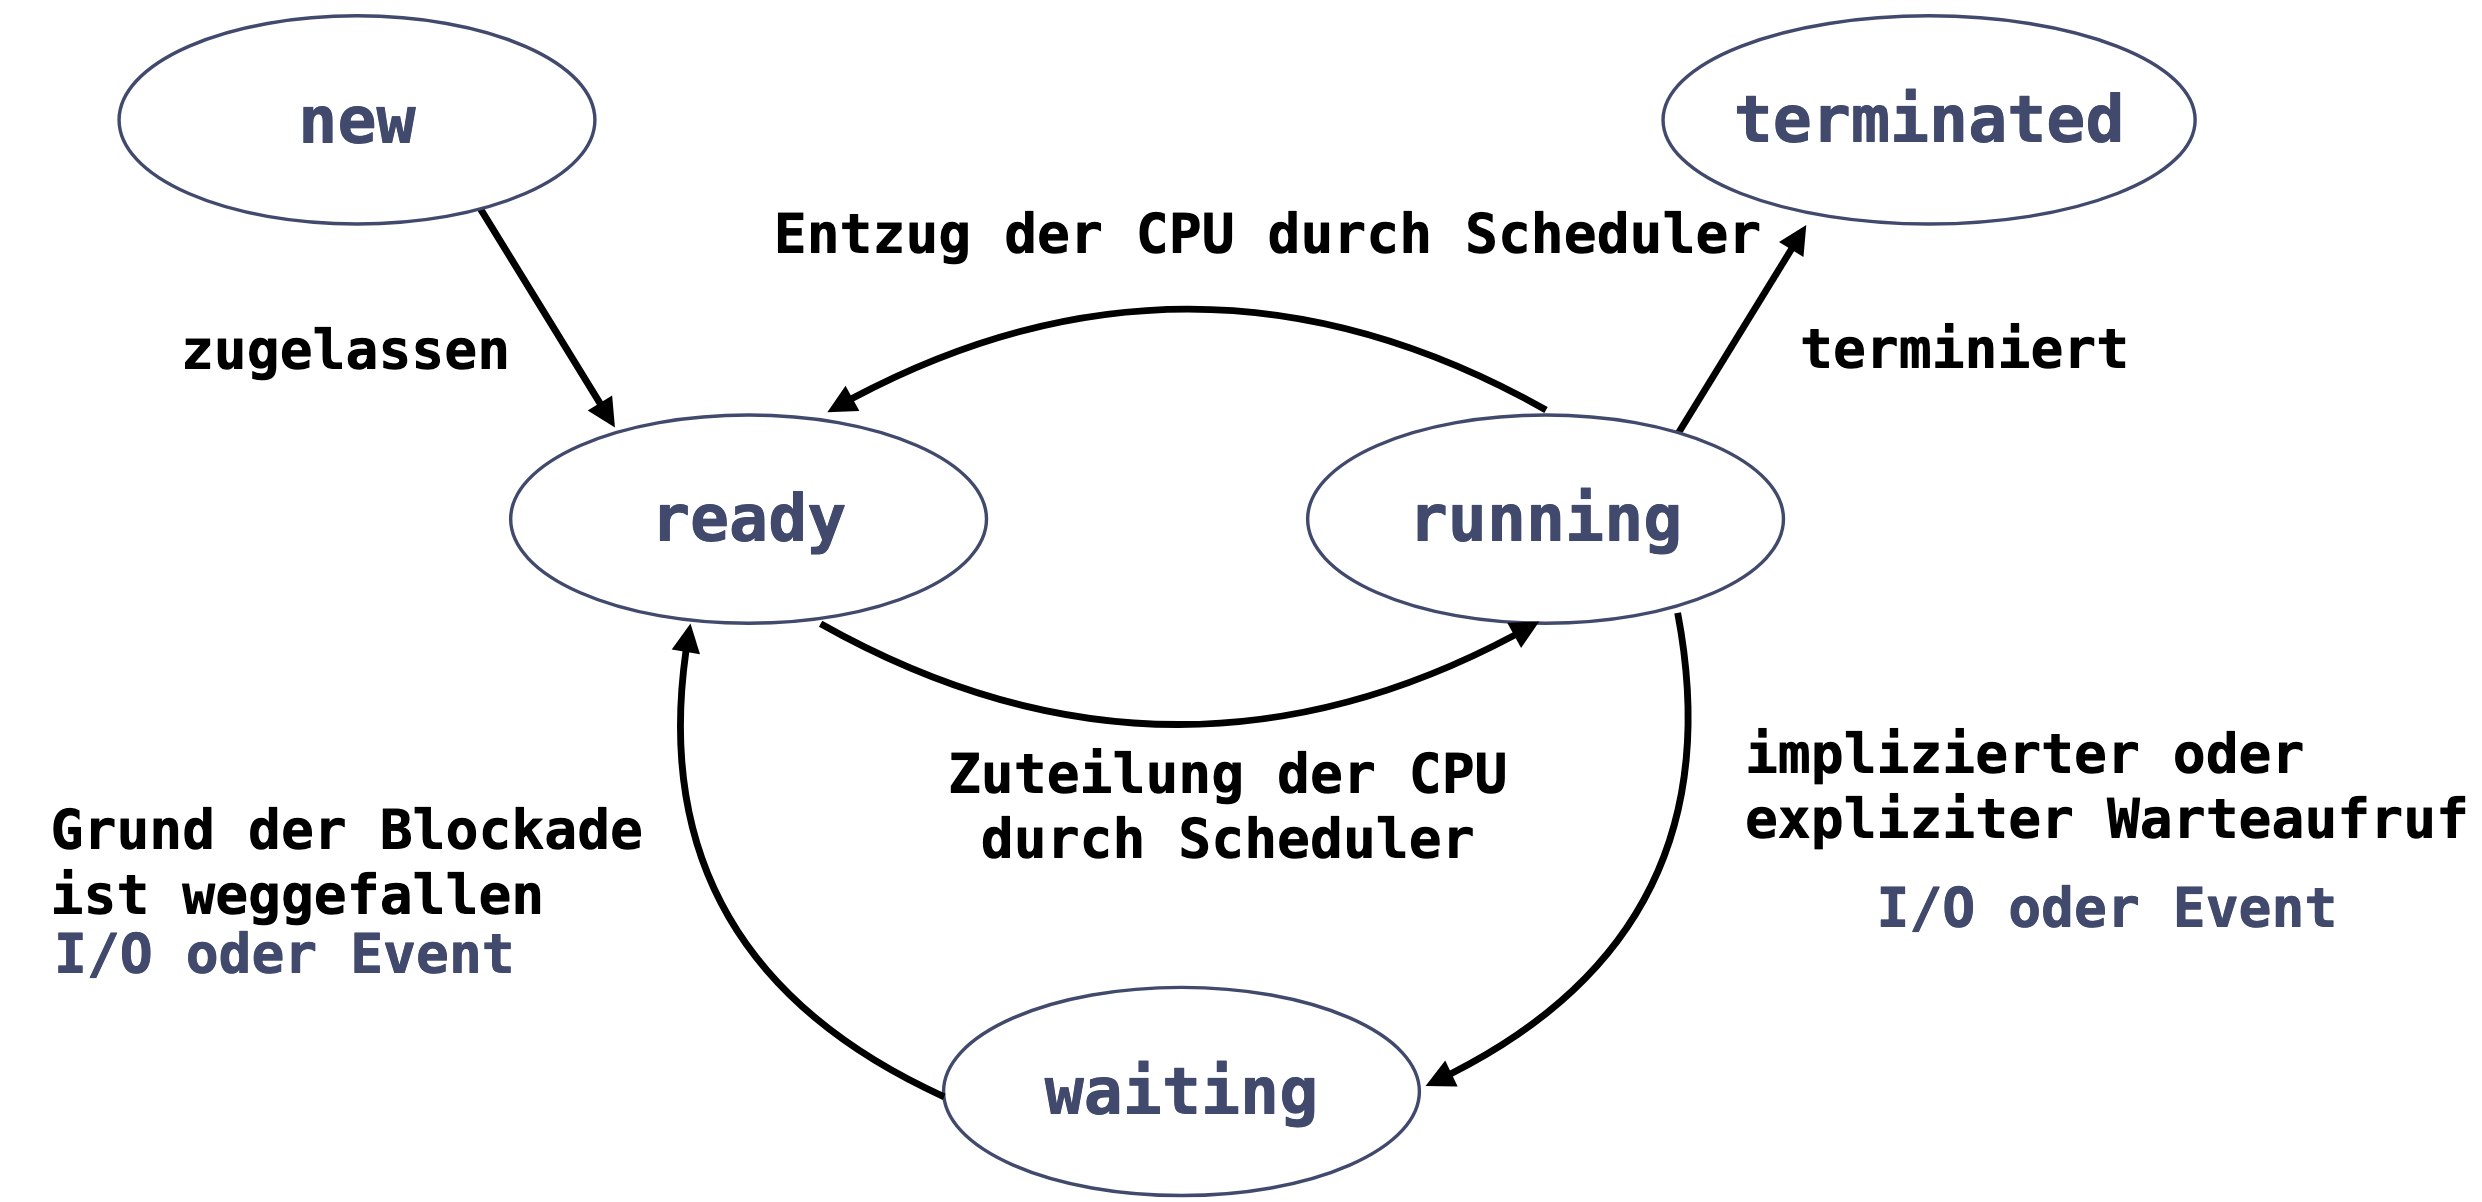
\includegraphics[scale=0.3]{Bilder/states.png}
	\caption{Eine Darstellung eines möglichen Prozessablaufs}
	\end{figure}
	
	Ein Prozess kann mehrere Zustände haben um weiderzugeben, was er momentan macht:
	\begin{itemize}
		\item{ready}
		\begin{itemize}
			\item{Der Prozess ist bereit die Ausführung fortzusetzen}
		\end{itemize}
		\item{running}
		\begin{itemize}
			\item{Der Prozess führt gerade in der CPU eine Funktion aus}
		\end{itemize}
		\item{waiting}
		\begin{itemize}
			\item{Der Prozess wartet auf eine spezifische Aktion oder eine spezifische Zeit}
		\end{itemize}
		\item{new}
		\begin{itemize}
			\item{Der Prozess wurde gerade erstellt}
		\end{itemize}
		\item{terminated}
		\begin{itemize}
			\item{Der Prozess hat seine Aufgabe beendet}
		\end{itemize}
	\end{itemize}
	Im Normalfall wechselt ein Prozess zwischen \verb|ready|  und \verb|running| . Wenn der Prozess darauf wartet, Prozessorzeit zugeteilt zu bekommen, ist er auf \verb|ready| . Wenn er gerade ausgeführt wird, ist er \verb|running| . Falls ein I/O Event oder ein sleep command dazu führt, dass der Prozess seine Ausführung unterbricht, ist er \verb|waiting|. Wenn ein Prozess gerade gestartet ist und noch keine Aufgabe getätigt hat, ist er new. Wenn der Prozess beendet wurde oder ans Ende seiner Ausführung gekommen ist, ist er \verb|terminated|. 
	\section{Einheit 2 - Scheduling}
	Ein Betriebssystem verwendet Scheduling um die Quasiparallelität der CPU zu erreichen. Dies macht der Umstand, dass eine CPU nur einen Auftrag gleichzeitig bearbeiten kann, nötig. Dabei wird eine ready queue erstellt, welche erfasst, welcher Prozess als nächstes dran ist. \\
	\begin{itemize}
		\item{Scheduler}
		\begin{itemize}
			\item{Entscheidet welcher Prozess als nächstes dran ist. Dies geschieht anhand einer Schedulingstrategie.}
		\end{itemize}
		\item{Dispatcher}
		\begin{itemize}
			\item{FÜhrt den Prozesswechsel durch. Er entzieht dem momentan laufenden Prozess auch die Berechtigung und erteilt sie dem Prozess, welcher in der Reihe an erster Stelle steht.}
			\item{Die Dispatch Latenz beschreibt hierbei die Zeit die benötigt wird um einen Prozess anzuhalten und einen anderen zu starten. Das Context Switching ist also nicht gratis}
			\begin{itemize}
				\item{So muss der Scheduler zuerst in den Kernel Modus wechseln, den Zustand des laufenden Prozesses speichern, den nächsten Prozess auswählen, die Umgebung für diesen Prozess laden und erneut in den User Modus wechseln.}
			\end{itemize}
		\end{itemize}
	\end{itemize}
	\subsection{Threads}
	Threads sind Ausführungen spezifischer Prozesse. So kann ein Prozess mehrere Threads haben, und diese teilen sich die Prozessumgebung mit Ausnahme des Stacksegments (Also gemeinsames Text-, Heap- und Datensegment). Threads bieten den Vorteil, dass sie bedeutend leichter zu wechseln sind, jedoch kann der geteilte Speicher zu anderen Problemen führen. \\
	Ein Context Switch kann in mehreren Fällen nötig sein. Wenn ein Prozess zum Beispiel beendet wird, muss ein Context Switch ausgeführt werden. Gleichzeitig kann es praktisch sein einen Context Switch zu vollführen, wenn der Prozess von running zu waiting wechselt, da der Prozess wahrscheinlich nicht sofort weiter ausgeführt werden muss. \\
	\subsection{Ziele}
	Scheduling hat das Ziel die CPU so sehr wie möglich auszulasten und somit die Illusion der Parallelität zu ermöglichen aber gleichzeitig so wenig wie möglich zu schedulen um die downtime des switchens zu verringern. \\
	Es gibt zwei große Wege Scheduling ausführen: Static und Dynamic \\
	Bei static scheduling wird im vorhinein entschieden wie viele cylces jeder Prozess bekommt. Dadurch können jedoch keine neuen Prozesse hinzugefügt werden, womit sie nur für integrierte Systeme sinnvoll sind. \\
	Dynamic Scheduling ist für nahezu alle anderen Systeme die bessere Methode. Bei diesen Methoden wird dynamisch festgelegt wie viele cycles diese zugesprochen kommen. Diese kann man wiederum in zwei Strategien teilen: Präemptive und nicht präemptive. \\
	\paragraphlb{Nicht Präemptives Scheduling}
	Hierbei wird der Prozess nicht von außen unterbrochen und ein Prozess kann so lange laufen, bis er beendet hat oder blockiert. Da man über diesen Prozess jedoch keine Kontrolle hat, ist es oft nicht sinnvoll.
	\paragraphlb{Präemptives Scheduling}
	Jeder Prozess bekommt eine gewisse Menge an Zyklen zugewiesen und danach wird der Prozess geändert. \\
	Ein paar Nicht Präemptive Schedulingstrategien sind:
	\begin{itemize}
		\item{First-come-first-served (FCFS)}
		\begin{itemize}
			\item{Der Prozess welcher zuerst eingereiht wurde, auch als erstes abgearbeitet wird. Dabei wird jeder neue Prozess an das Ende der Schlange gestellt. So wird ein First In, First Out realisiert (FIFO)}
		\end{itemize}
		\item{Shortest-Job-First Scheduling (SJF)}
		\begin{itemize}
			\item{Bei Wahl des nächsten Prozess wird immer der gewählt, dessen Laufzeit am geringsten ist. Dabei muss jedoch grundsätzlich im Vorhinein bekannt sein, wie lange der Prozess läuft. Das ist zwar oft nicht bekannt, jedoch kann man eventuell aus bisherigen Erfahrungen in etwa erahnen wie lange Prozesse laufen. Da es jedoch ein nicht präemptives Verfahren ist, muss, nachdem ein Prozess begonnen hat stets warten bis dieser beendet oder unterbricht. SJF ist auch nur optimal, wenn alle Prozesse gleichzeitig verfügbar sind und die Laufzeiten verfügbar sind bzw. die Annahmen gut sind.}
		\end{itemize}
	\end{itemize}
	Präemptive Schedulingstrategien sind:
	\begin{itemize}
		\item{Shortest-Time-Remaining (STR)}
		\begin{itemize}
			\item{Funktioniert gleich wie SJF, vergleicht jedoch stets wie lange der aktuelle Prozess noch brauchen wird und wie lange wartende Prozesse brauchen. Falls bei einem neuen Prozess angenommen wird, dass er weniger Zeit als der aktive benötigt, wird dieser unterbrochen und der neue Prozess stattdessen ausgeführt.}
		\end{itemize}
		\item{Round Robing}
		\begin{itemize}
			\item{Eine der am meistesten verwendeten Verfahren. Dabei wird reihum zugeteilt und jeder Prozess bekommt einen spezifische Menge an Zyklen, before der nächste Prozess an der Reihe ist. Dabei wird der CPU auch ein neuer Prozess zugeteilt wenn der Prozess beendet oder er auf etwas wartet. Die Effizienz dieser Strategie hängt davon ab wie effektiv die Länge der Zeitscheibe gewählt wird. Wenn sie zu kurz ist, wird viel Zeit durch Context Switches verschwendet. Wenn sie jedoch zu lange ist, gibt es effektiv keinen Unterschied zu dem FCFS Verfahren.}
		\end{itemize}
		\item{Präemptives Priority Scheduling}
		\begin{itemize}
			\item{Hierbei wird ein Prozess anhand der Wichtigkeit zuerst abgearbeitet. Ein Emailprogramm hat zum Beispiel eine geringere Priorität, als andere Programme, weil es normalerweise nicht ersichtlich ist, ob die Email eine Sekunde später empfangen wird.}
			\item{Man kann hierbei jedoch auch zwischen einer Präemptiven und einer Nicht Präemptiven unterscheiden. Bei einer Nicht Präemptiven wird die Queue stets nach priorität gereiht, und abgearbeitet aber kein Prozess unterbrochen. Bei Präemptiven wird der aktive Prozess unterbrochen falls ein Prozess mit einer höheren Priorität auftaucht.}
			\item{Prioritäten können in zwei Wegen zugewiesen werden: Statisch oder Dynamisch. Bei statischer Priorität wird die Priorität eines Prozesses am Anfang des Prozesslebens zugeteilt und verändert sich nie. Dadurch kann es jedoch passieren, dass sehr niedrigrelevante Prozesse nie zum Zug kommen. \\
			Um sowas zu verhindern gibte es dynamische Prioritätenzuweisung und ein Prozess, welcher die CPU mehr benötigt, wird in der Priorität abgestuft (Aging) oder ein Prozess, welcher seit längerem wartet wird aufgewertet.}
		\end{itemize}
		\item{Multilevel Feedback Queue Scheduling}
		\begin{itemize}
			\item{Bei diesem Verfahren werden mehrere Queues generiert, welche unabhängig eigene Schlangen bilden. Jede dieser Schlangen hat dabei eine andere Priorität. Nachdem ein Prozess CPU Zeit erhalten hat, wird dieser danach oft in eine niedrigere Priorität gereiht. Mit der Zeit werden auch Prozesse, welche länger keine CPU Time erhalten haben, höhergestuft um sicherzustellen, dass sie nicht zu lange inaktiv bleiben (starvation).}
		\end{itemize}
		\item{Completely Fair Scheduler}
		\begin{itemize}
			\item{Der Scheduler welcher von Linux benutzt wird. Dabei wird jedem Prozess \textit{virtual runtime} (vruntime) zugewiesen und eingestuft anhand wie viel CPU Zeit die Prozesse bereits erhalten haben.}
		\end{itemize}
	\end{itemize}
	 \section{Einheit 3 - 25.11.2024}
	 \subsection{Prozesskommunikation}
	 Es ist oft vonnöten, dass Prozesse miteinander kommunizieren. Das ist nicht nur in Fällen, wichtig, in welchen Prozesse Informationne austauschen müssen, sondern auch die sichere Verwendung von Ressourcen, welche von beiden Prozessen benötigt werden oder die korrekte Ausführung von Prozessen, welche von anderen Prozessen abhängig sind. Prozesse haben mehrere Wege um so Informationen auszutauschen:
	 \begin{itemize}
	 	\item{Pipe}
	 	\begin{itemize}
	 		\item{Unidirektionaler Kanal zwischen zwei Prozessen. Prozess A schreibt Daten in den Kanal und Prozess B kann diese auslesen.}
	 	\end{itemize}
	 	\item{Prozeduraufrufe (Remote Procedure Calls)}
	 	\begin{itemize}
	 		\item{Ein Prozess ruft eine Prozedur oder Funktion eines anderen Prozesses auf und kann so interagieren.}
	 	\end{itemize}
	 	\item{Gemeinsame Dateien oder ein gemeinsamer Speicherbereich}
	 	\begin{itemize}
	 		\item{Prozesse teilen sich Dateien oder Speicherbereiche und können diese gemeinsam benutzen und verändern.}
	 	\end{itemize}
	 \end{itemize}     
	 \subsubsection{Race Conditions}
	 Wenn sich zwei Prozesse Ressourcen teilen, kann es eventuell passieren, dass beide Prozesse "gleichzeitig" auf eine Variable zugreifen und es so zu Inkonsistenzen in den Daten kommt. Auch wenn solche Fälle nur sehr selten auftreten, ist die Ursache für Fehler, welche als Konsequenz geschehen nur sehr schwer aufzuspüren. Solch ein Szenario kann man jedoch vermeiden, indem nie zwei Prozesse die gleiche Variable verändern kann. \\
	 \paragraphlb{Producer-Consumer-Beispiel}
	 Ein solcher Fall könnte in einem Beispiel passieren, in welchem es einen Konsumenten und einen Produzenten. Beide Parteien haben Zugriff auf ein Array, nehmen jedoch andere Rollen ein. Um die Größe des Arrays im Blick zu behalten, wird eine Variable \verb|count|  verwendet, welche die Anzahl der Elemente enthält. Der Konsument kann dabei, falls das Array nicht leer ist, ein Element aus dem Array entfernen und den \verb|count| um 1 zu verringern. Der Produzent hingegen kann, falls das Array \textbf{nicht voll} ist, ein Element dem Array hinzufügen und den \verb|count| um 1 zu erhöhen. Falls jedoch nun beide Parteien gleichzeitig den count verändern wollen, kann es passieren, dass ein context switch geschieht, nachdem eine Partei den neuen \verb|count| berechnet, ihn jedoch noch nicht abgespeichert hat. Wenn nun die andere Partei während des context switches \verb|count| auch verändern will, geht diese Veränderung verloren, da der zuvor berechnete Wert die neue Veränderung nicht berücksichtigt. \\
	 Ein solches Problem nennt man eine \textbf{race condition}. Dadurch hängt das Ergebnis einer Operation vom zeitlichen Verhalten einer Einzeloperation ab. Wenn also zwei oder mehr Prozesse gemeinsamen Speicher lesen, kann das Endergebnis von dem CPU Scheduling abhängen. Eine weitere Ursache kann der Umstand sein, dass eine Gruppe an Befehlen nicht als unteilbar angegeben werden. Wenn man zum Beispiel \verb|count++| eingibt, wird das innerhalb des Prozesses in drei Befehle gespalten, welche danach Opfer einer race condition werden können. 
	 \paragraphlb{Synchronisation}
	 Um solche race conditions zu verhindern, muss man sicherstellen, dass Prozesse miteinander synchronisiert werden. Ein Weg um dies zu erreichen ist die Definition von \textbf{critical regions}. Diese Regionen können dadurch jeweils nur von einer Partei gleichzeitig beschrieben werden um so sicherzustellen, dass kein anderer Prozesse im falschen Moment eine Variable überschreibt. Wenn ein Prozess dann in eine kritische Region eintritt und währenddessen pausiert wird, wird ein anderer Prozess davon abgehalten die Variable zu verändern und stattdessen deaktiviert, bis die kritische Region von dem anderen Prozess wieder verlassen wurde.\\
	 Es gibt drei Möglichkeiten so einen wechselseitigen Ausschluss zu implementieren:
	 \begin{itemize}
	 	\item{Deaktivieren von Interrupts}
	 	\begin{itemize}
	 		\item{Wenn ein Prozess einen kritischen Abschnitt betritt, werden interrupts ausgeschalten. So wechselt die CPU nicht zu einem anderen Prozess, während dieser kritische Bereich besetzt ist.}
	 		\item{Dies ist zwar eine einfache Lösung, kann jedoch sehr gefährlich werden, da man einem Prozess nicht vertrauen sollte.}
	 		\item{Findet vielleicht Anwendung in Situationen, wo keine fremde Software ausgeführt wird.}
	 	\end{itemize}
	 	\item{Striktes Alternieren (Spinlock)}
	 	\begin{itemize}
	 		\item{Wenn ein Prozess einen kritischen Abschnitt betreten will, dieser jedoch blockiert ist, wartet er bis er nicht mehr blockiert ist.}
	 		\item{Diese Strategie verbraucht jedoch CPU Zeit während der Prozess auf die Blockierung wartet.}
	 	\end{itemize}
	 	\item{Mutex (\textit{Mut}ual \textit{Ex}clusion)}
	 	\begin{itemize}
	 		\item{Jeder kritische Bereich besitzt eine Variable, welche entweder blockiert oder nicht blockiert sein kann.}
	 		\item{Falls ein Prozess einen kritischen Bereich betreten will, dieser jedoch blockiert ist und \verb|blocked| erhält, wird er schlafen gelegt, bis der Bereich wieder frei ist.}
	 		\item{Alle modernen Betirebssysteme verwenden Mutex.}
	 	\end{itemize}
	 \end{itemize}
	 Der Unterschied zwischen einem Spinlock und einem Mutex ist, dass bei einem Spinlock der Prozess wartet und weiter CPU Zeit verbraucht, während er auf das Ende der Blockade wartet, während ein Mutex den Prozess schalfen legt, bis der Bereich nicht mehr blockiert ist und dadurch keine CPU Zeit verbraucht.
	 \subsubsection{Deadlock}
	 Wenn jedoch zwei Prozesse jeweils aufeinander warten, kann dies zu einer Verklemmung führen, oft \textit{Deadlock} genannt. Es gibt einige Situationen, in welchen so etwas vorkommen kann, hat jedoch bei mutex' eine besondere Relevanz. Damit es zu einem Deadlock kommen kann, müssen 4 Voraussetzungen erfüllt sein:
	 \begin{itemize}
	 	\item{Wechselseitiger Ausschluss - Jede Resource ist entweder verfügbar oder genau einem Prozess zugeordnet.}
	 	\item{Hold-and-wait - Ein Prozess, welcher Ressourcen reserviert hat, kann weitere Ressourcen anfordern.}
	 	\item{Ununterbrechbarkeit - Ressourcen die einem Prozess bewilligt wurden, können nicht wieder vom Betriebssystem entzogen werden.}
	 	\item{Zyklische Wartbedingung - Es muss eine zyklische Liste geben, sodass ein Prozess jeweils auf einen anderen Prozess in der Liste warten kann.}
	 \end{itemize}
	 \paragraphlb{Behandlung}
	 Man kann solch einen Deadlock auf verschiedene Weisen auflösen:
	 \begin{itemize}
	 	\item{Erkennen und Beheben}
	 	\begin{itemize}
	 		\item{Ein Betriebssystem lässt einen deadlock zwar zu, behebt es jedoch danach indem es einen der Prozesse beendet. Diese Strategien wie der Wait Graph, welcher ein Netz aus wartenden Prozessen spannt, sind jedoch meist sehr aufwändig und ressourcenintensiv.}
	 	\end{itemize}
	 	\item{Vermeidung}
	 	\begin{itemize}
	 		\item{Da für einen Deadlock stets die 4 Voraussetzungen gegeben sein müssen, kann man einen deadlock vermeiden indem man zumindest eine davon verhindert.}
	 		\item{Zum Beispiel könnte das Betriebssystem verlangen, dass ein Prozess am Anfang jeglichen Speicher anfordert.}
	 		\item{Ebenfalls könnte ein Programm erneut mittels Wait Graph eine angeforderte Ressource nicht freigeben, wenn es wahrscheinlich ist, dass dies einen Deadlock verursachen könnte.}
	 	\end{itemize}
	 	\item{Ignorieren}
	 	\begin{itemize}
	 		\item{Eine weitere Möglichkeit ist es, einen Deadlock zu ignorieren und so darauf zu warten, dass der Benutzer das Programm manuell beendet.}
	 		\item{Da deadlocks sehr selten sind und es für den Benutzer oft schnell ersichtlich wird, dass das Programm feststeckt, verzichten moderne Betriebssysteme oft auf aufwändige Algorithmen zur Erkennung von Deadlocks.}
	 	\end{itemize}
	 \end{itemize}
	 \subsection{Hauptspeicherverwaltung}
	 \subsubsection{Flüchtigkeit}
	 Grundsätzlich unterscheidet man zwischen flüchtigem und nicht flüchtigem Speicher. Flüchtiger Speicher behält seinen Wert nur solange er mit Spannung versorgt wird. Der RAM als Primärspeicher ist ein flüchtiger Speicher. Großer Vorteil ist dabei, dass er einen zufälligen Zugriff ermöglicht und deshalb unabhängig von der gesuchten Speicherzelle eine konstante Zugriffszeit hat. Im Gegensatz dazu hält sich nicht-flüchtiger Speicher selbst nachdem es ihre Spannung verloren hat. Nicht-flüchtiger Speicher wird meist als Festplatte in Systemen verwendet und ist im Fall von älteren mechanischen Speichermedien wie HDDs, Disketten und Kassetten sequenziell, muss also durchlaufen werden um eine bestimmte Speicherzelle zu finden. \\
	 In modernen Systemen unterscheidet man in sechs verschiedene Speichersysteme, welche anhand ihrer Größe und Zugriffszeit sortiert werden:
	 \begin{itemize}
	 	\item{Register}
	 	\begin{itemize}
	 		\item{Kleinster Speicher mit in der Regel nur ein paar KByte an Speicher. Extrem schnelle Zugriffszeiten (~{}100 ps)}
	 	\end{itemize}
	 	\item{Cache}
	 	\begin{itemize}
	 		\item{Puffer Speicher, welcher zwischen Arbeitsspeicher und Prozessor liegt. Im Schnitt nur ein paar MByte groß und einer Zugriffszeit von ~{}1 ns}
	 	\end{itemize}
	 	\item{Hauptspeicher}
	 	\begin{itemize}
	 		\item{Da Register und Cache sehr beschränkt in ihrer Kapazität sind, müssen Daten im Hauptspeicher zwischengespeichert werden. Drastisch größerer Speicher als Cache und Register (8 - 16 GByte) aber auch bedeutend langsamerer Zugriffszeiten. (~{}10 ns)}
	 	\end{itemize}
	 	\item{Festplatte}
	 	\begin{itemize}
	 		\item{Dient als langfristiger Speicher für Daten aus dem Hauptspeicher. Bietet wiederum größere Kapazität (1 TByte+) und langsamerer Zugriffszeiten (~{}10 ms)}
	 	\end{itemize}
	 	\item{CD-ROM/DVD/BlueRay}
	 	\begin{itemize}
	 		\item{Wird als extern verfügbarer Speicher verwendet. Bietet in der Regel weniger Speicher als die Festplatte (50 GByte) ist jedoch wechselbar.}
	 	\end{itemize}
	 	\item{Magnetband}
	 \end{itemize}
	 \paragraphlb{Register}
	 \paragraphlb{Cache}
	  Hardware überprüft ob ein Block im cache liegt. Cache-Hit falls vorhanden und Cache-Muss falls nicht.
	 \paragraphlb{Hauptspeicher}
	Nach der von Neumann Architektur werden sowohl Daten als auch das Programm im Hauptspeicher gespeichert. Aus diesem Grund muss man sicherstellen, dass ein Programm nicht fremde Daten oder den Code eines anderen Programms verändert. \\
	Im Hauptspeicher müssen Daten als Bitfolgen abgespeichert werden. Dabei wird unterschieden ob diese in Little Endian oder Big Endian gespeichert werden. Little Endian speichert hierbei Dies entscheidet ob die Bytes von oben nach unten oder unten nach oben gelesen werden müssen. \\
	Es muss auch überwacht werden, dass der Arbeitsspeicher organisiert ist. Dafür ist der Memory Manager verantwortlich. Dieser optimiert die CPU-Auslastung und Computerantwortzeit. So koordiniert er die gemeinsame Verwendung des Hauptspeichers und teilt so Prozessen Hauptspeicher zu, verwaltet freien Speicher und implementiert Schutzmechanismen für Speicherzugriff. Ebenso stellt er den virtuellen Speicher zur Verfügung damit jedes Programm nicht wissen muss in welcher Speicherzelle es liegt.\\
	Bei der Speicherverwaltung muss man zwischen realem und virtuellem Speicher unterscheiden. 
	\subsubsection{Realer Speicher}
	\paragraphlb{Monoprogrammierung}
	Im Falle des realen Speichers gibt es die Monoprogrammierung, in welchem nur ein Prozess sowie das Betriebssystem existieren. Das ist wünschenswert, wenn das System nur eine Aufgabe zu erfüllen hat, was auch die Speicherveraltung sehr einfach macht. Falls mehr als 1 Prozess existiert, kann man mittels Swapping den Speicher für ein Programm jeweils zwischen dem Arbeitsspeicher und der Festplatte wechseln.
	\paragraphlb{Feste Partitionierung}
	Bei der festen Partitionierung wird der Speicher in verschiedene Speicherblöcke geteilt, welche unterschiedliche Größen haben können. Pro Partition ist ein Prozess erlaubt wodurch unterschieden werden kann, welcher Teil des Speichers welchem Prozess gehört. Es gibt eine Schlange pro Partition und wird zugewiesen sobald der nächste Prozess an der Reihe ist. Diese Strategie ist relativ Platzineffizient, da nicht jeder Prozess die gleiche Menge an Speicher benötigt, die Partitionen jedoch eine feste Größe haben. Man darf jedoch die Partitionen auch nicht zu klein machen, da sonst viele Prozesse diesen nicht verwenden können.\\
	Wenn ein Prozess weniger Speicher benötigt, als die Partition groß ist, kann der restliche Speicher nicht mehr verwendet werden, bis ein neuer Prozess in der Partition diesen zusätzlich zum Rest der Partition benötigt. Diese Lücken innerhalb der Partitionen nennet man \textbf{Interne Fragmentierung/Verschnitt}. \\
	Da es mehrere Prozesse innerhalb des Speichers gibt, muss man einen Speicherschutz implementieren. Dabei wird meist das Base/Limit System verwendet. Dabei hat jede Partition eine Base Zelle, welche die untere Grenze des Speichers darstellt und das Limit, welches zum base addiert wird um die höchstmögliche Zelle für diese Partition festzustellen.
	\paragraphlb{Dynamische Speicherzuteilung}
	Ein weiteres System ist die dynamische Speicherzuteilung. Dabei weist das Betriebssystem dynamisch Speicherbereiche zu, welcher im Optimalfall aufeinanderfolgend ist. Das System muss dabei Allokation und Freigabe verwalten. \\
	\begin{figure}[H]
	\centering
	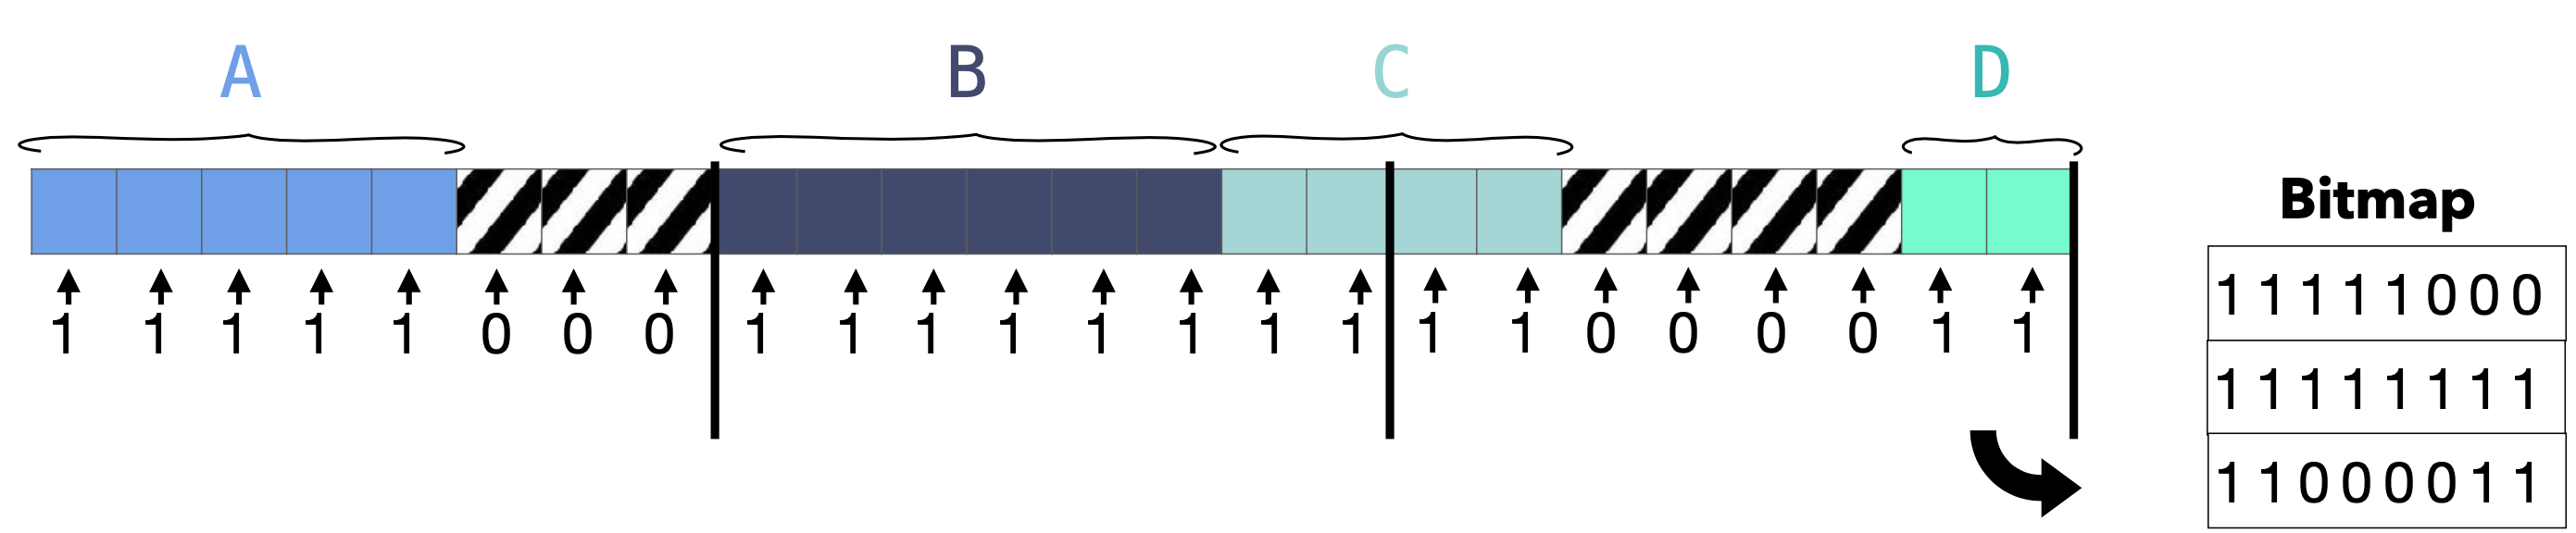
\includegraphics[scale=0.38]{Bilder/bitmap.png}
	\caption{Eine Repräsentation einer bitmap}
	\end{figure}
	Da der Speicher dynamisch zugeteilt wird, muss das BS zu jedem Zeitpunkt wissen wem welche Speicherzelle zugeteilt wurde und welche frei ist. Das System kann hierbei den Speicher in Zuteilungsblöcke unterteilen, zum Beispiel mittels Bitmaps oder verketteten Listen. Bitmaps sind Repräsentationen von Einsen und Nullen (Zum Beispiel in einem Bild). Diese Bitmaps zeigen im Speicher an, welche Einheit belegt (1) und welche frei (0) ist. Da das System den Speicher dynamisch angibt, kann so effizient Speicher in Blöcken zugeteilt werden. Im Gegensatz zur festen Partitionierung kann Speicher, welcher von einem Prozess nicht vollständig gebraucht wird, stattdessen diesen an einen anderen Prozess vergeben. Dieses System wird in Unix/Linux verwendet.
	\begin{figure}[H]
	\centering
	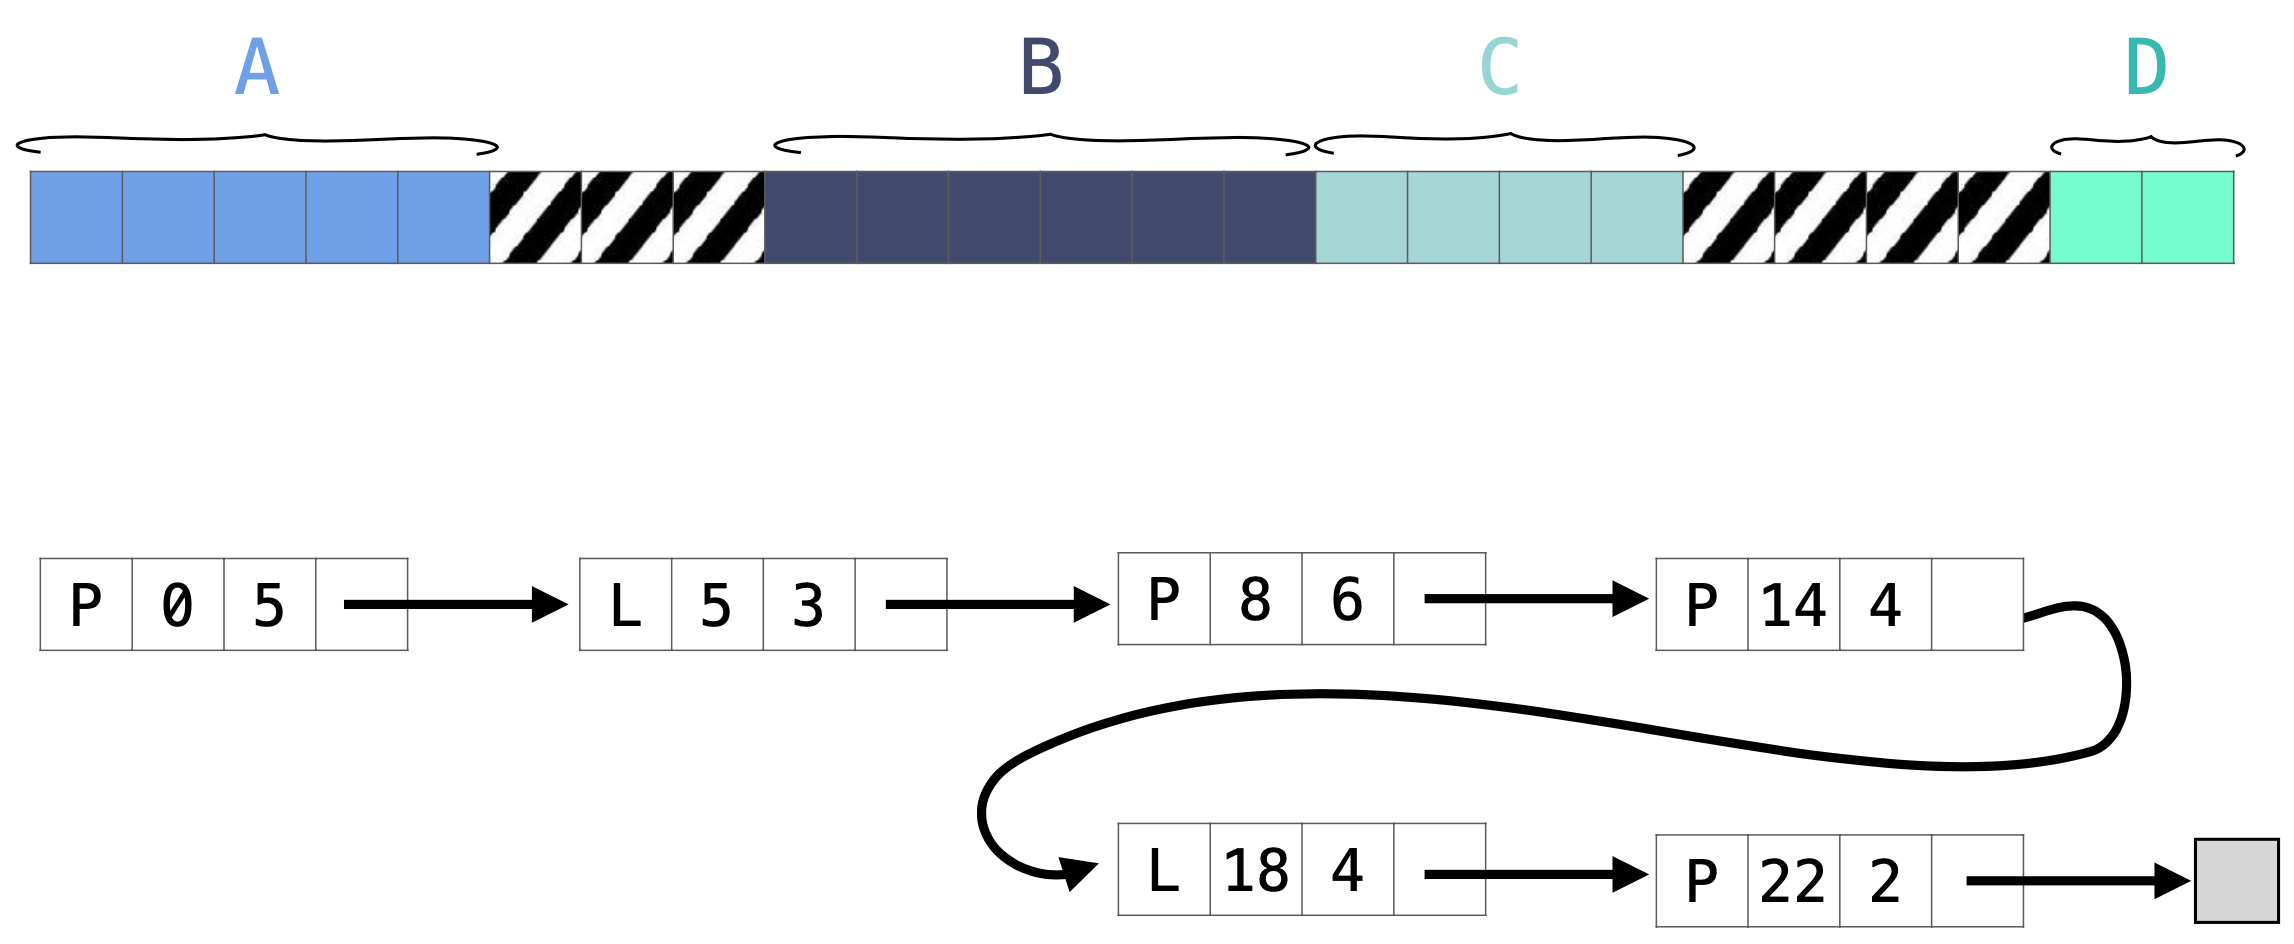
\includegraphics[scale=0.4]{Bilder/linkedlist.png}
	\caption{Eine Respräsentation einer verketteten Liste}
	\end{figure}
	Verkettete Listen geben stattdessen am Anfang an, wie viele Einheiten belegt sind, und verweisen auf das nächste Element. So kann eine Liste zum Beispiel so aussehen: \verb|P-0-5-(Verweis auf das nächste Element)|. P gibt an, dass das Segment einen Prozess enthält, 0 zeigt den Anfang der Adresse und 5 das Ende, sowie ein Verweis auf das nächste Segment. \\
	\paragraphlb{Fitting}
	Es gibt mehrere Strategien diesen Speicher dynamisch zu füllen:
	\begin{itemize}
		\item{First Fit}
		\begin{itemize}
			\item{Der Speicher wird von Anfang an durchlaufen und der erste passende Speicherblock wird gewählt (Selbst wenn er zu groß ist.)}
		\end{itemize}
		\item{Next Fit}
		\begin{itemize}
			\item{Anstatt jedes Mal wieder von Anfang an zu beginnen, sucht Next Fit ab der letzten gefundenen Speicherstelle.}
		\end{itemize}
		\item{Best Fit}
		\begin{itemize}
			\item{Durchläuft den gesamten Speicher und wählt dann den besten Block.}
		\end{itemize}
		\item{Worst Fit}
		\begin{itemize}
			\item{Durchläuft auch den gesamten Speicher wählt jedoch dann den größten Speicherblock. (Damit auch große Blöcke verwendet werden.)}
		\end{itemize}
		\item{Quick Fit}
		\begin{itemize}
			\item{Unterhält zwei verkettete Listen, jeweils für Prozesse und für Lücken. Danach muss nur die Liste der Lücken durchlaufen werden um schnell alle freien Speicherstellen zu finden.}
		\end{itemize}
	\end{itemize}
	Bei dieser Speicherstrategie kann es jedoch auch zu einer Fragmentierung kommen, und zwar der externen Fragmentierung. Da Speicher jeweils dynamisch vergeben wird, kann es sein, dass ein Block belegt wird und dadurch ein Segment hinterlässt, welches zu klein ist um einen weiteren Prozess zu halten. Dieser Block wird dadurch höchstwahrscheinlich nicht verwendet bis einer der angrenzenden Prozesse wieder freigegeben wird.
	\subsubsection{Buddy Zuteilungssystem}
	Linux verwendet ein System namens Buddy. Dabei versucht die Speicherverwaltung stets einen Block so passend wie möglich zu verteilen. Um dies zu erreichen spaltet das System den Speicher into Blöcke, welche jeweils Zweierpotenzen darstellen. Wenn das System also nur 1024KB zur Verfügung hat, und ein Prozess 100KB benötigt, spaltet das System Blöcke bis ein Block 128KB hat, da eine weitere Spaltung mit 64KB zu klein wäre. Dadurch wird in etwa stets der effektivste Block zugeteilt. \\
	\subsubsection{Speicherüberlastung}
	Da der Arbeitsspeicher nur eine begrenzte Größe hat, wird dessen Größe oft nicht ausreichen um alle möglichen Programmdaten zu halten. Um trotzdem alle Prozesse bearbeiten zu können, kann man mittels swapping den Speicher in der Festplatte und den Speicher im RAM auszutauschen. Dabei wird Speicher aus dem RAM auf die Festplatte ausgelagert und eingelagert. Dieser Prozess ist jedoch relativ ineffizient, da die Schreib- und Lesegeschwindigkeit im Vergleich zum RAM relativ begrenzt ist (~{}100MB/s).
	\section{Virtueller Speicher}
	Im realen Speicher gilt die Regel, dass ein Programm vollständig im Speicher vorhanden sein muss, bevor es ausgeführt werden kann. Es kann jedoch passieren, dass ein Programm zu groß ist, um komplett im Arbeitsspeicher Platz zu finden. Dabei wird virtueller Speicher relevant, welcher ermöglicht, dass ein Prozess nicht komplett geladen werden muss um trotzdem ausführbar zu sein. Im virtuellen Speicher wird jedem Prozess vorgespielt, dass der gesamte Arbeitsspeicher nur ihm zur Verfügung steht. Da die Verbindung zwischen dem Speicher, der einem Prozess zur Verfügung steht und dem echten Speicher, so schwächer ist, kann ein Programm auch in mehreren Teilen über den Arbeitsspeicher verteilt sein. Das ist auch eine Möglichkeit wie Systeme mit virtuelleme Speicher eine Speicherüberlastung umgehen können.
	\subsection{Memory Management Unit (MMU)}
	Um diese realen Adressen mit den virtuellen Adressen verbinden zu können, wird die MMU verwendet. Sie behält einen Index beider Adresswelten und übersetzt einen in das andere. Ist oft ein dezidierter Chip um hohe Geschwindigkeiten zu garantieren. Dieser Chip meldet auch Zugriffsverletzungen, wenn ein Prozess außerhalb seiner Zugriffsrechte agieren will.
	\subsection{Abstraktion}
	Bei einem virtuellen Speicherblock, wird jedem Prozess ein Adressraum zugewiesen. Jeder Prozess hat in seinem eigenen Adressraum vermeintlich unendlich viel Speicher zu Verfügung, welcher von dem Betriebssystem bei Bedarf stets erweitert wird. In modernen Betriebssystemen arbeitet kein Prozess mehr mit realen Adressen, sondern nur mehr mit virtuellen Adressen. Lediglich der Boot Runner beim Starten des Systems arbeitet noch mit realem Speicher. Da die virtuellen Adressen keine direkte Relation zu dem realen Speicher haben, kann sich ein Teil des Programms somit auch auf einem Sekundärspeicher befinden, welcher bei Bedarf von dem Betriebssystem in den Arbeitsspeicher geladen wird.
	\subsubsection{Logische Adressraumbelegung}
	Der Speicher wird in separate logische Adressräume geteilt, welche jeweils verschiedene Anwendungszwecke haben.
	\begin{itemize}
		\item{Text oder Code}
		\begin{itemize}
			\item{Beinhaltet den ausführbaren Programmcode}
		\end{itemize}
		\item{Daten}
		\begin{itemize}
			\item{Beinhaltet globale Variablen mit unbeschränkter GÜltigkeitsdauer}
		\end{itemize}
		\item{Heap}
		\begin{itemize}
			\item{Dynamisch zugeteilter Speicher (Objekte wie String Variablen)}
		\end{itemize}
		\item{Stack}
		\begin{itemize}
			\item{Auch dynamisch und beinhaltet lokale Daten mit beschränkter Gültigkeitsdauer. (Wie lokale Variablen)}
		\end{itemize}
	\end{itemize}
	\begin{figure}[H]
	\centering
	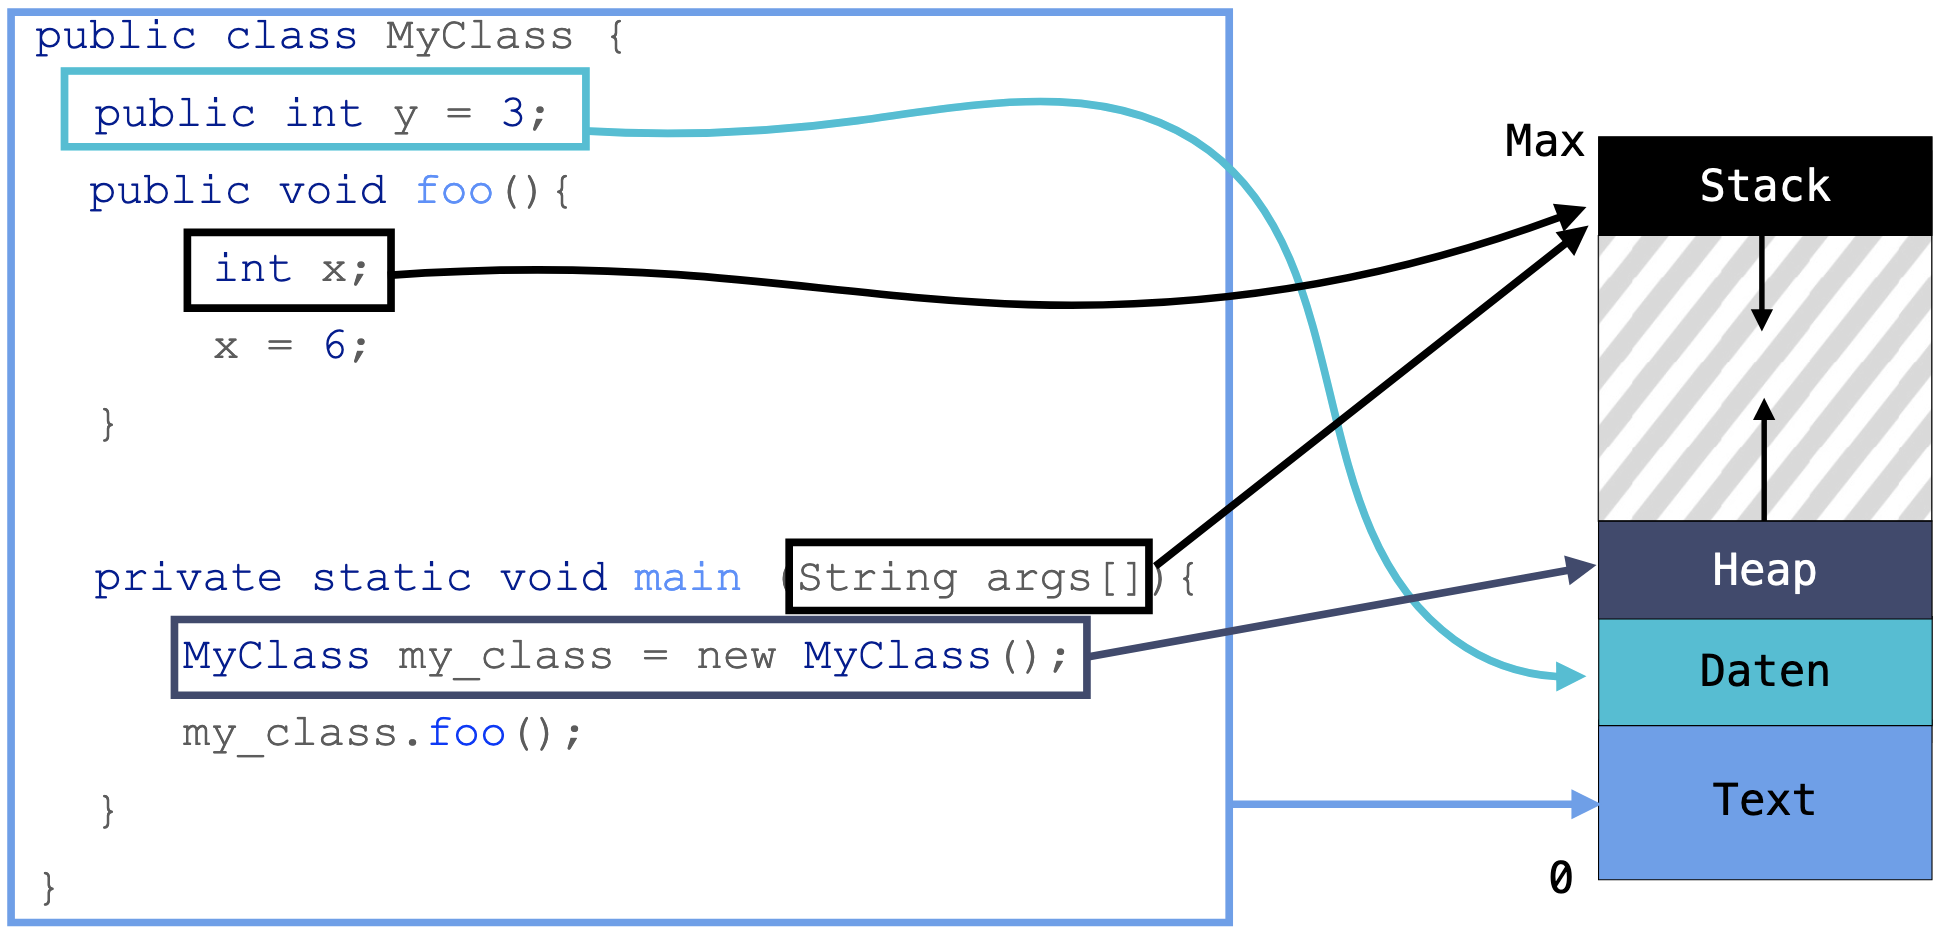
\includegraphics[scale=0.3]{Bilder/virtual.png}
	\caption{Programmcode und ihr Aufenthaltsort}
	\end{figure}
	Es mag hier scheinen, als ob der gesamte Speicher eine Einheit bilden, er kann jedoch in unterschiedlichen Segmenten im Speicher existieren.
	\subsection{Paging}
	Virtueller Adressraum wird in Pages eingeteilt, welche jeweils die gleiche Größe haben. Jede Seite ist dabei ein aneinander grenzende Bereiche von Adressen eingeteilt. Die Größer einer solchen Page ist variabel und kann zwischen 512 Byte und 1GB liegen, ist jedoch typischerweise 4KB groß. Es ist jedoch wichtig, dass jede Seite innerhalb des Speichers die gleiche Größe hat. Eine virtuelle page wird dabei im physikalischen Raum in einer page frame gespeichert. Ein Prozess namens \textit{Demand Paging} ermöglicht hierbei, dass ein Prozess nicht komplett im Speicher vorhanden sein muss um ihn auszuführen. Der Ort der einzelnen Seiten wird dabei mittels Page Table festgehalten.
	\subsubsection{Page Table}
	Wird verwendet um eine Page zu einem Page Frame zu übertragen. Dabei hält die Page Table den Aufenthaltsort der Page im physischen Speicher, sowie dessen virtuelle Speicheradresse fest. \\
	Dabei enthält jede Page Table stets:
	\begin{itemize}
		\item{Die Seitennummer}
		\begin{itemize}
			\item{Die virtuelle Adresse der Page}
		\end{itemize}
		\item{Eine Seitenrahmen Nummer}
		\begin{itemize}
			\item{Die physische Repräsentation der Page im Page Frame}
		\end{itemize}
		\item{Zustand der Seite (Present-Bit)}
		\begin{itemize}
			\item{Hält fest ob diese Page verwendet wird. \verb|0 -> Nicht vorhanden, 1 -> Vorhanden|}
		\end{itemize}
		\item{Zusatzinformation (Zetstempel für letzte Nutzung, Einlagerung, Ändern ...)}
	\end{itemize}
	\begin{figure}[H]
	\centering
	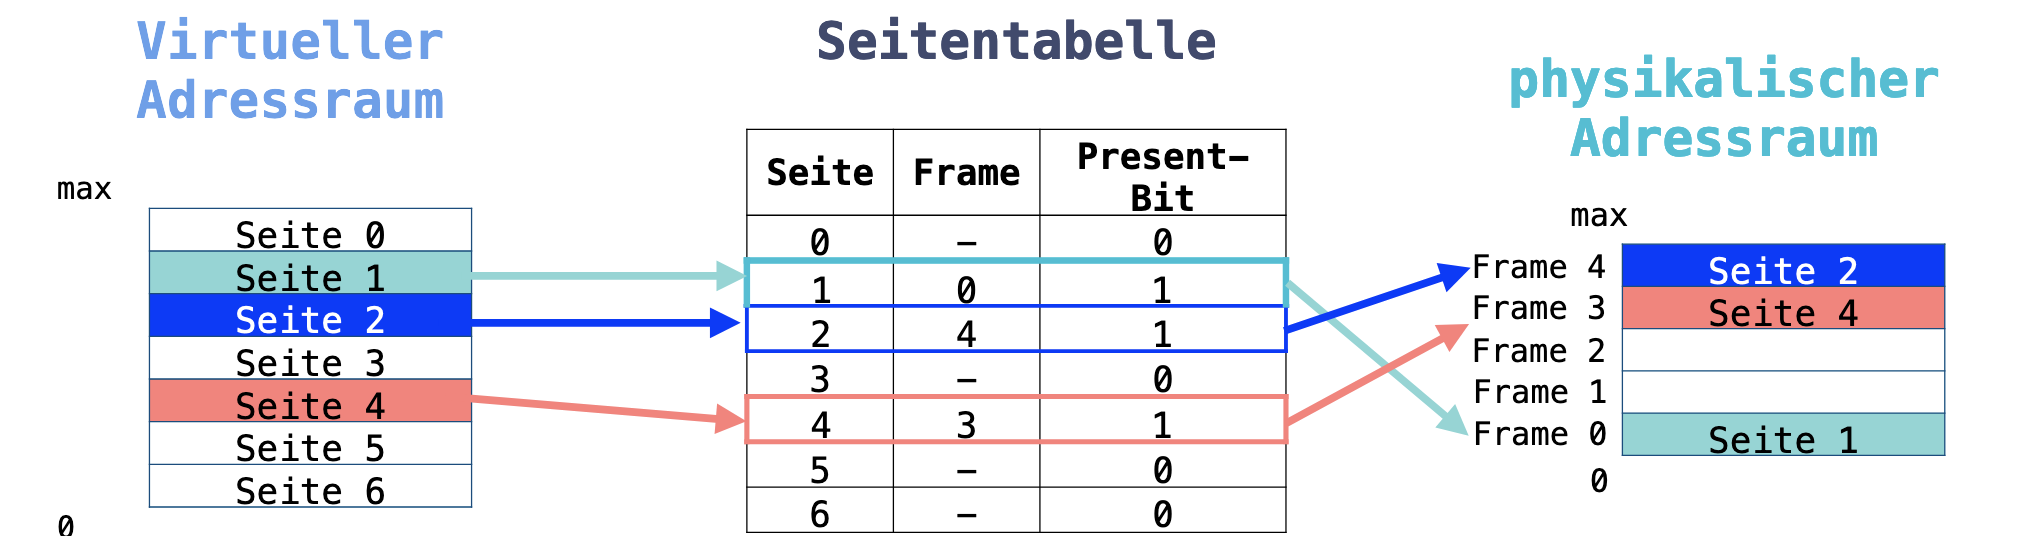
\includegraphics[scale=0.5]{Bilder/pagetable.png}
	\caption{Übersetzung der Page in einen Page Frame anhand der Page Table}
	\end{figure}
	Die physikalische Adresse besteht aus der Summe der Physical Frame Number und dem Offset innerhalb der Page
	\subsubsection{Zugriffsszenarien}
	Bei einer Zugriffsanfrage gibt es zwei mögliche Ausgänge:
	\paragraphlb{Ein Prozess will auf Speicher zugreifen, der im physischen Speicher vorhanden ist.}
	\begin{tabular}{| l | l | l |}
		\toprule
		Seite & Frame & Present-Bit \\ \midrule
		1 & - & 0 \\ \hline
		1 & 0 & 1 \\ \hline
		2 & 3 & 1 \\ \hline
		3 & - & 0 \\ \hline
		4 & 2 & 1 \\ \hline
		5 & - & 0 \\ \hline
		6 & - & 0 \\
		\bottomrule
	\end{tabular} \\
	Gegeben ist folgende Tabelle. Dabei sind sowohl VPN als auch PFV 4 Bit Zahlen. Zusätzlich gibt es im Arbeitsspeicher 4 Frames \verb|-> {0, 1, 2, 3}| \\
	\textbf{\small{Übersetze die virtuelle Adresse in eine physische}} \\
	a) \verb|0010 1110 -> Logische Adresse [VPN + Offset]| \\
	Man muss die VPN Nummer links (0010) in Dezimal übersetzen (2) und die Seitennummer in der Tabelle mit der Frame Nummer (3) in Binär (0011) übersetzen. Der Offset ist in beiden Fällen gleich und bleibt bestehen. Der Offset ist hierbei die Zeilennummer innerhalb der Page (Also kann es innerhalb einer Page mehrere Offsets geben) \\
	\verb|0011 1110 -> Physische Adresse [PFN + Offset]|
	\paragraphlb{Ein Prozess will auf Speicher zugreifen, der \textbf{nicht} im physischen Speicher vorhanden ist.}
	Wenn keine gültige Zuordnung besteht, tritt ein \verb|Page Fault| auf. Dabei wird die Übersetzung abgebrochen und stattdessen versucht die Page im physischen Speicher einzulagern. Die MMU nimmt so einen freien Page Frame und ordnet ihm der neuen Page zu.
	\paragraphlb{Ein Prozess will auf Speicher zugreifen, der \textbf{nicht} im physischen Speicher vorhanden ist, es existiert jedoch kein freies Frame}
	Wenn keine Frame verfügbare ist, muss eine sogenannte Opferseite gefunden werden. Das ist eine Page, welche in den Sekundärspeicher ausgelagert werden soll, um Platz für die neue Page zu schaffen. Dabei gibt es drei Strategien um ein Frame zur Auslagerung zu bestimmen:
	\begin{itemize}
		\item{First in - First Out (FIFO)}
		\begin{itemize}
			\item{Der schon am längsten im Hauptspeicher existierende Frame wird ausgelagert.}
			\item{Kann problematisch sein, da der älteste Frame nicht unbedingt ein unbedeutender ist.}
		\end{itemize}
		\item{Least Recently Used (LRU)}
		\begin{itemize}
			\item{Die Seite die am längsten nicht genutzt wurde, wird ausgelagert}
		\end{itemize}
		\item{Second Chance}
		\begin{itemize}
			\item{Kombiniert die anderen zwei Verfahren und entfernt die älteste Seite, die nicht genutzt wurde.}
		\end{itemize}
	\end{itemize}
	\subsubsection{Translation Lookaside Buffer (TLB)}
	Da die Umrechnung der virtuellen Adressen sehr schnell erfolgen muss, gibt es einen Cache zur Speicherung von oft verwendeten Adresspaaren. Das Nachsehen in dem TLB ist schneller als die Übersetzung des MMUs, da der Lookaside Buffer keine Berechnungen vornimmt um die Adressen zu ermitteln sondern nur die Referenz einer Adresse, auf eine andere speichert. Nur wenn im TLB kein passendes Paar zur Verfügung steht, wird die MMU zur Rate gezogen. Der Zugriff auf die TLB ist extrem schnell, da diese Paare in einer Hash Tabelle gespeichert werden, wodurch sie in nahezu konstanter Zeit gefunden werden können. Dabei agiert die Ursprungsadresse als Key, und die Zieladresse als Value (In Key:Value Paaren).


	
	















\end{document}